
\documentclass[twoside,twocolumn]{article}
\usepackage{amsmath}
\usepackage{blindtext} % Package to generate dummy text throughout this template 
\usepackage{graphicx}
\usepackage{natbib}

\usepackage[sc]{mathpazo} % Use the Palatino font
\usepackage[T1]{fontenc} % Use 8-bit encoding that has 256 glyphs
\linespread{1.05} % Line spacing - Palatino needs more space between lines
\usepackage{microtype} % Slightly tweak font spacing for aesthetics

\usepackage[english]{babel} % Language hyphenation and typographical rules

\usepackage[hmarginratio=1:1,top=32mm,columnsep=20pt]{geometry} % Document margins
\usepackage[hang, small,labelfont=bf,up,textfont=it,up]{caption} % Custom captions under/above floats in tables or figures
\usepackage{booktabs} % Horizontal rules in tables

\usepackage{lettrine} % The lettrine is the first enlarged letter at the beginning of the text

\usepackage{enumitem} % Customized lists
\setlist[itemize]{noitemsep} % Make itemize lists more compact

\usepackage{abstract} % Allows abstract customization
\renewcommand{\abstractnamefont}{\normalfont\bfseries} % Set the "Abstract" text to bold
\renewcommand{\abstracttextfont}{\normalfont\small\itshape} % Set the abstract itself to small italic text

\usepackage{titlesec} % Allows customization of titles
\renewcommand\thesection{\Roman{section}} % Roman numerals for the sections
\renewcommand\thesubsection{\roman{subsection}}
\titleformat{\section}[block]{\large\scshape\centering}{\thesection.}{1em}{} % Change the look of the section titles
\titleformat{\subsection}[block]{\large}{\thesubsection.}{1em}{} % Change the look of the section titles

\usepackage{fancyhdr} % Headers and footers
\pagestyle{fancy} % All pages have headers and footers
\fancyhead{} % Blank out the default header
\fancyfoot{} % Blank out the default footer
\fancyhead[C]{FYS4150 $\bullet$ Project 1 $\bullet$ September 2016} % Custom header text
\fancyfoot[RO,LE]{\thepage} % Custom footer text

\usepackage{titling} % Customizing the title section

\usepackage{hyperref} % For hyperlinks in the PDF

%----------------------------------------------------------------------------------------
%	TITLE SECTION
%----------------------------------------------------------------------------------------

\setlength{\droptitle}{-4\baselineskip} % Move the title up

\pretitle{\begin{center}\Huge\bfseries} % Article title formatting
\posttitle{\end{center}} % Article title closing formatting
\title{FYS4150 - Project 1} % Article title
\author{%
\textsc{Heine H. Ness \& Sindre R. Bilden} \\[1ex] % Your name
\normalsize University of Oslo \\ % Your institution
\normalsize \href{mailto:h.h.ness@fys.uio.no}{h.h.ness@fys.uio.no}\ ; \href{mailto:s.r.bilden@fys.uio.no}{s.r.bilden@fys.uio.no}\\% Your email address
\normalsize \href{https://github.com/sindrerb/FYS4150-Collaboration}{github.com/sindrerb/FYS4150-Collaboration}
%\and % Uncomment if 2 authors are required, duplicate these 4 lines if more
%\textsc{Jane Smith}\thanks{Corresponding author} \\[1ex] % Second author's name
%\normalsize University of Utah \\ % Second author's institution
%\normalsize \href{mailto:jane@smith.com}{jane@smith.com} % Second author's email address
}
\date{\today} % Leave empty to omit a date
\renewcommand{\maketitlehookd}{%
\begin{abstract}

\noindent In physics one usually describes nature by using a mathematical models. The differential equation is one of the most common ways to describe dynamical phenomena in nature. They are usually on the form $-u''(x)=f(x)$ and some of the more famous ones are so hard to solve that they are practically impossible to solve analytically. Luckily mankind has invented the transistor and from it we have created the computer which allows the use of numerical methods to get an approximate solution for some of the harder  differential equations.
\nl
In this exercise we solve one of these famous equations using three different approaches. This way we see how it benefits us to think ahead before using well known methods such as \textit{LU-decomposition} to power trough a problem. We also see how the number of floating point operations has a significant impact on how much time is used solving a given problem. And we see how close to an analytical solution the numerical approximation really gets. 

\end{abstract}
}

\newcommand{\nl}{

\medskip
\noindent
}

%----------------------------------------------------------------------------------------

\begin{document}

% Print the title
\maketitle

%----------------------------------------------------------------------------------------
%	ARTICLE CONTENTS
%----------------------------------------------------------------------------------------

\section{Introduction}

\lettrine[nindent=0em,lines=3]{M}any formulas in physics are differential equations. Some of these are not solveble analytically but by numerical methods an approximation close to the exact solution may be achieved. A broad selection of  numerical methods have been designed throughout time, where all have their different strengths and weaknesses.
In this project we have examined three different techniques for approximating the solution to a particular differential equation where a continuous function is known.\nl 

The chosen equation - Poisson equation - describes an electrostatic potential $\Phi$ generated by a localized charge density $\rho(\vec{r})$ and is usually described - in three dimensions - by:
\begin{equation}
\nabla^2\Phi = -4\pi \rho(\vec{r}) \label{eq:Poisson3D}
\end{equation}
If $\rho(\vec{r})$ is spherical symmetric, eq. \ref{eq:Poisson3D} may be written in a one-dimensional manner by substituting $\phi(r)=r\Phi(r)$:
\begin{equation}
\frac{d^2\phi(r)}{dr^2}=-4\pi r\rho(r) \label{eq:Poisson1D}
\end{equation}
By rewriting eq. \ref{eq:Poisson1D} to a general form it reads:
\begin{equation}
-u''(x)=f(x) \label{eq:general}
\end{equation}
In this specific case, the Poisson equation is solved by \textit{LU-decomposition} (LU) and later compared to a more suited method called \textit{Thomas method}, both in a general manner and an optimized way for one spessific matrix.

%------------------------------------------------
\section{Methods}
The mathematical and nummerical methods used in this projects are the following:
\begin{itemize}
\item Dirichlet boundary conditions
\item Numerical derivation
\item Thomas algorithm
\item LU-decomposition
\item Numerical error analysis
\end{itemize}

\subsection{Dirichlet boundary condition}
Dirichlet boundary conditions - also referred to as fixed boundary condition - specifies the value of a given function on a surface $T=f(r,t)$. In a one-dimensional problem it translates to defining an interval of $x$ - $x\in [x_{min},x_{max}]$ - and the function values $f(x_{min})=f_{low}$ and $f(x_{max})=f_{high}$ at the edges of the interval.

\subsection{Numerical derivation}
The derivative of a discrete function may be found by numerical derivation. The principle of numerical derivation is a result of Taylor expansion. By expanding a function from a point $x$ with a step $h$, two equations form depending on the direction of the step:
\begin{equation}
f(x+h) = f(x)+hf'(x)+\frac{h^2}{2}f''(x)\ldots \label{eq:taylor_pos}
\end{equation}
\begin{equation}
f(x-h) = f(x)-hf'(x)+\frac{h^2}{2}f''(x)\ldots \label{eq:taylor_neg}
\end{equation}
By adding eq. \ref{eq:taylor_neg} to eq. \ref{eq:taylor_pos}, a approximation for the second derivative is achieved.
\begin{equation}
f'' = \frac{f_+-2f+f_-}{h^2}+\frac{h^4}{6h^2}f^{\mathit{IV}}\label{eq:sec_der}
\end{equation}
Where $f_+ = f(x+h)$, $f=f(x)$, $f_-=f(x-h)$ and $f^{IV}$ is the fourth derivative of $f(x)$. By truncating the series at the fourth derivative a small mathematical error appears in the order of $h^2$. If a discrete function is introduced where $f_i = f(x_i) = f(x_0+ih)$, eq. \ref{eq:sec_der} may be rewritten to an algorithm for the numerical second derivative.
\begin{equation}
f''_i = \frac{f_{i+1}-2f_i+f_{i-1}}{h^2}\label{eq:sec_der_discrete}
\end{equation}
In eq. \ref{eq:sec_der_discrete} the mathematical error $\mathcal{O}(h^2)$ is neglected.

\subsection{Thomas algorithm}
Thomas algorithm is a variant of Gaussian elimination used on tridiagonal matrices \cite{compfys}, where Gaussian elimination is a method using $\mathcal{O}(n^3)$ floating point operations (FLOPS) for solving a set of $n$ linear equations with $n$ unknown variables $x_i$ $i=0,1,\ldots,n-1$. Thomas algorithm is usefully applied if the equations is on the form :
\begin{align*}
a_{i}x_{i-1}+b_{i}x_i+c_{i}x_{i+1}&=y_i
\end{align*}
Resulting in a matrix equation $\hat{A}x= y$ where $\hat{A}$ and $y$ is known.
\begin{equation*}
\begin{bmatrix}
b_1&c_1&0&\cdots &0\\
a_2&b_2&c_2& \ddots & \vdots\\
0&a_3&b_3&\ddots&0\\
\vdots&\ddots&\ddots&\ddots&c_{n-1}\\
0&\cdots&0&a_n&b_n
\end{bmatrix}
\begin{bmatrix}
x_1\\x_2\\x_3\\x_4\\\vdots\\x_{n}
\end{bmatrix}=
\begin{bmatrix}
y_1\\y_2\\y_3\\y_4\\\vdots\\y_{n}
\end{bmatrix} 
\end{equation*}
Both Thomas algorithm and Gaussian elimination is divided into two main parts, forward and backward substitution.

\subsubsection{Forward substitution}

The forward substitution is focusing on reducing the number of elements in a column to a minimum. In other words, row reduction is first used on the matrix $\hat{A}$ to eliminate all elements $a_{i}$. Turning the matrix equation to $\hat{B}x=\tilde{y}$:
\begin{equation*}
\begin{bmatrix}
b_1&c_1&0&\cdots &0\\
0&\tilde{b}_2&c_2& \ddots & \vdots\\
0&0&\tilde{b}_3&\ddots&0\\
\vdots&\ddots&\ddots&\ddots&c_{n-1}\\
0&\cdots&0&0&\tilde{b}_n
\end{bmatrix}
\begin{bmatrix}
x_1\\x_2\\x_3\\x_4\\\vdots\\x_{n}
\end{bmatrix}=
\begin{bmatrix}
\tilde{y}_1\\\tilde{y}_2\\\tilde{y}_3\\\tilde{y}_4\\\vdots\\\tilde{y}_{n}
\end{bmatrix} 
\end{equation*}
where $\tilde{b}$ and $\tilde{y}$ is affected by the row reduction. The new set of linear equations is the basis for backward substitution.

\newpage
\subsubsection{Backward substitution}

The concept of backwards substitution is to solve the the set of equations from bottom to top. The bottom $x$ can be expressed as $x_n=\frac{\tilde{y}_n}{\tilde{b}_n}$ and may be used to solve the equation above. In the end, all elements of $x$ is known. In total, the Thomas algoritm is using $9n$ FLOPS. If the matrix elements is constant through every diagonal, the number of FLOPS may be reduced to $4n$.

\subsection{LU-decompostition}
LU decomposition (LU) also known as LU- , Crout or Dolittle factorisation \cite{linalg:lay}\cite{compfys} is a common way to solve matrix problems numerically. It is used to find important matrix properties such as the determinant.
\nl
Most importantly it reduces the number of FLOPS used to solve linear algebra problems, from 
$\mathcal{O}(n^3)$ FLOPS by a regular Gaussian elimination to $\mathcal{O}(n^2)$ by LU-decomposition \cite{compfys}.
\nl
LU-decomposition as the name suggests decomposes a matrix $\hat{A}$ into two matrices $\hat{L}$ and $\hat{U}$ where $\hat{L}$ is a lower triangular matrix with ones along its diagonal and $\hat{U}$ is an upper triangular matrix. For this to be possible $\hat{A}$ needs to be a square, invertible matrix.

\begin{align*}
&\hat{A}= 
\begin{bmatrix}
a_{11}&a_{12}&\cdots &a_{1n}\\
a_{21}&a_{22}& \cdots & a_{2n}\\
\vdots&\vdots&\ddots&\vdots\\
a_{n1}&a_{n2}&\cdots&a_{nn}
\end{bmatrix}=\hat{L}\hat{U}=\\
&\begin{bmatrix}
1&0&\cdots &0\\
L_{21}&1& \cdots & 0\\
\vdots&\vdots&\ddots&\vdots\\
L_{n1}&L_{n2}&\cdots&1
\end{bmatrix}
\begin{bmatrix}
U_{11}&U_{12}&\cdots &U_{1n}\\
0&U_{22}& \cdots & U_{2n}\\
\vdots&\vdots&\ddots&\vdots\\
0&0&\cdots&U_{nn}\end{bmatrix} 
\end{align*}

All elements in $\hat{L}$ and $\hat{U}$ are found by calculating one column at a time starting with column one and proceeding in an increasing fashion. Here $j$ represents the column number.
First all elements $U_{1j}$ is found by

\begin{equation*}
    U_{1j} = a_{1j}    
\end{equation*}

Then compute $U_{ij}$ with $i = 2,3,\cdots,j-1$

\begin{equation*}
    U_{ij} = a_{ij}-\sum_{m=1}^{i-1}L_{im}U_{mj} 
\end{equation*}

Then the diagonal elements $U_{jj}$ is found by

\begin{equation*}
    U_{jj} = a_{jj}-\sum_{m=1}^{j-1}L_{jm}U_{mj} 
\end{equation*}

Lastly the $L_{ij}$ where $i>j$ is calculated

\begin{equation*}
    L_{ij} = \frac{1}{U_{jj}}\left(a_{ij}-\sum_{m=1}^{i-1}L_{im}U_{mj}\right)
\end{equation*}

For more details see reference \cite{compfys}.

\subsection{Numerical error estimate}
Since numerical methods are used, the result is only an approximation to the analytical answer.
Therefore it is interesting to see how good the numerical method is by comparing the approximation to an already known solution.    
A good way to do this is to look at the relative error $\varepsilon_r$ between the approximation and the exact solution. At small step lengths $h$, the approximation is often close to the exact solution if the theory is correct. Therefore it is convenient too look at the logarithm of the relative error to differentiate methods of nearly equal accuracy. An appropriate formula is:
\begin{equation}
\varepsilon_i = \log_{10}\left(\left|\frac{v_i - u_i}{u_i}\right|\right)\label{eq:num_err}
\end{equation}
Where $v_i$ is the numerical value and $u_i$ is the analytical value at step $i$.

\newpage

\section{Implementation}

By discretizing the simplified and generalized Poisson equation (eq. \ref{eq:general}) in steps of $h$, we may use eq. \ref{eq:sec_der_discrete} to write eq. \ref{eq:sec_der_num} where $v_i$ is the numerically approximated discrete values for the continuous analytical function $u(x)$.
\begin{equation}
-\frac{v_{i+1}-2v_i+v_{i-1}}{h^2}=f_i \label{eq:sec_der_num}
\end{equation}
The equation may be rewritten into a linear equation
\begin{equation*}
av_{i-1}+bv_i+cv_{i+1}=\tilde{b}_i 
\end{equation*}
where $a=-1$, $b=2$, $c=-1$ and $\tilde{b}_i=f_ih^2$. By introducing Dirichlet boundary conditions, $v_0=v_{n+1}=0$, the linear equations may be written in terms of matrix multiplication without loss of information. This results in $Av=\tilde{b}$:
\begin{equation}
\begin{bmatrix}
b&c&0&0&\cdots &0\\
a&b&c&0& \cdots & 0\\
0&a&b&c& \cdots & 0\\
\vdots&\vdots&\vdots&\vdots&\ddots&c\\
0&0&0&0&a&b
\end{bmatrix}
\begin{bmatrix}
v_1\\v_2\\\vdots\\v_{n-1}\\v_{n}
\end{bmatrix}=
\begin{bmatrix}
\tilde{b}_0\\\tilde{b}_1\\\vdots\\\tilde{b}_{n-2}\\\tilde{b}_{n-1}
\end{bmatrix} \label{eq:problem}
\end{equation}
The problem is now solvable by both LU-decomposition and Thomas algorithm. Since matrix $A$ has a constant value along it's diagonals, an optimized Thomas algorithm was constructed to this specific matrix.
In this assignment $f(x)$ and its solution $u(x)$ were given as described below. And all programs were tested against the solution.

\begin{equation*}
f(x)=100\exp[-10x]
\end{equation*}
\begin{equation*}
u(x)=1-\exp[-10]x-10\exp[-10x]
\end{equation*}
For all programs, divided in task $b$, $c$, $d$ and $e$ see the github repository: 

\begin{center}
 \href{https://github.com/sindrerb/FYS4150-Collaboration}{github.com/sindrerb/FYS4150-Collaboration}
\end{center}

\newpage

\section{Results and discussion}

\subsection{LU-decomposition}

Solving eq. \ref{eq:problem} using LU-decomposition works on each element in the whole matrix and does not take in to consideration the trigonal nature of the problem it is then a more time consuming process than necessary. It is also often a non-satisfying method for square matrices of size above $10^4$ due to limits in memory. Table \ref{tbl:time_LU} shows the computation time for a set of matrices of size $N$.

\begin{table}[h]
\begin{tabular}{|l|l|l|l|l|} \hline
$N$ & 1e1 & 1e2 & 1e3 & 1e4\\ \hline
t [s] & 2.78e-4 &4.62e-3 & 8.198e-1 & 8.614e2\\ \hline
\end{tabular}
\caption{Table showing computation time $t$ in seconds for LU-decompositon of matrices of size $N$.} \label{tbl:time_LU}
\end{table}

All LU calculations were done using the Armadillo library for C++ \cite{arma}.

\subsection{General Thomas algorithm}

Solving eq. \ref{eq:problem} by the more suited Thomas algorithm reduced the computation time significantly compared to the LU-decomposition. Thomas method gave a - by eye - satisfying approximation at 100 iterations, as seen in Figure \ref{fig:Thomas1E2}. Although - by investigating the numerical error analysis - the increased number of iterations shows a significant increase of accuracy up to $N=10^6$ iterations, at higher number of iterations the accuracy seems to drop as seen i Table \ref{tbl:error}.
The algorithm seems to have a tendency to underestimate the derivative and will approach the exact solution from below at a low number of iterations, as seen in Figure \ref{fig:Thomas10}.

\begin{table}[htp]
\centering
\begin{tabular}{|l|l|} \hline
Iterations & Relative error\\ \hline
1e1 & -1.17970\\
1e2 & -3.08804\\
1e3 & -5.08005\\
1e4 & -7.07927\\
1e5 & -9.07909\\
1e6 & -10.7943\\
1e7 & -9.54215\\ \hline
\end{tabular}
\caption{Table showing the relative error from Thomas method based on eq. \ref{eq:num_err} for a set of iterations.}\label{tbl:error}
\end{table}


The reduction of accuracy at $n=10^7$ iterations  is most likely caused by loss of precision in the numerical derivation. $n=10^7$ iterations leads to a step-length $h\simeq 10^{-7}$ which gives terms of $f_(i)$ close to each-other. The term $f_{i+1}-2f_i+f_{i-1}$ could be the source of precision loss if the differences in $f_i$ is in order of $\sim10^{-15}$

\begin{figure}[htp]
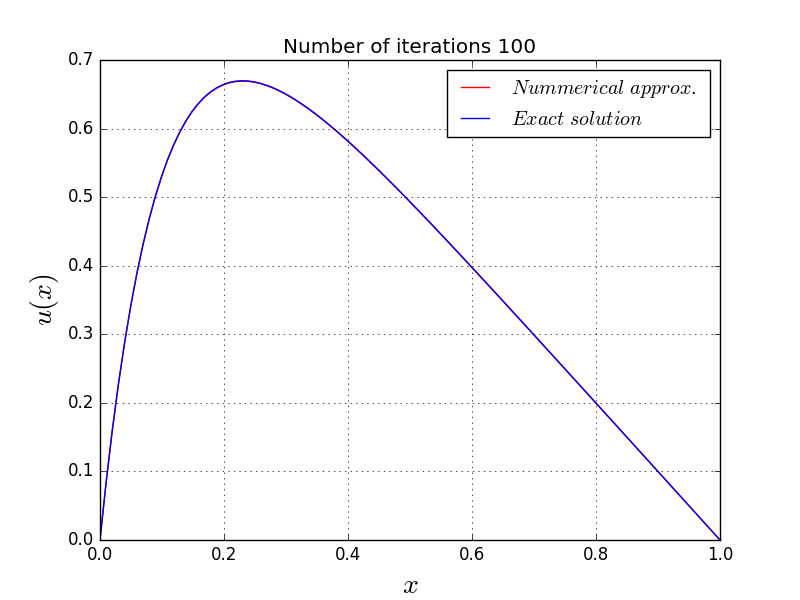
\includegraphics[width=0.5\textwidth]{figures/b-run1e2.png} 
\caption{Plot of the numerical approximation of $u(x)$ - in red - with 100 iterations by Thomas algorithm, compared to the exact solution $u(x)$ in blue.} \label{fig:Thomas1E2}
\end{figure}

\begin{figure}[htp]
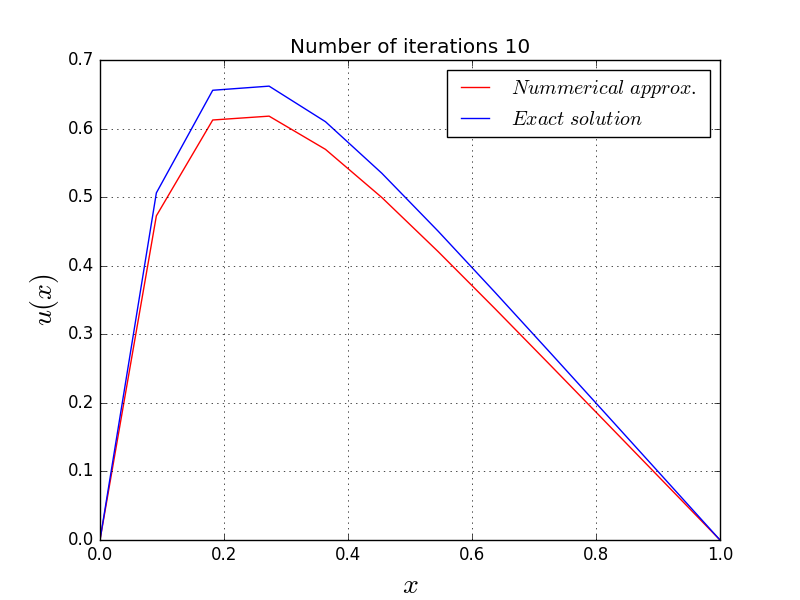
\includegraphics[width=0.5\textwidth]{figures/b-run10.png} 
\caption{Plot of the numerical approximation of $u(x)$ - in red - with 10 iterations by Thomas algorithm, compared to the exact solution $u(x)$ in blue.} \label{fig:Thomas10}
\end{figure}


\subsection{Specialized Thomas algorithm}
Solving eq. \ref{eq:problem} with a specialized Thomas algorithm gave - as expected - the same results as the general algorithm, but reduced the number FLOPS from $9n$ in the general algorithm to $4n$ in the specialized algorithm. The reduction in number of FLOPS shorted the commutation time. A difference in the computation time is hard to spot at a low number of iterations, but a higher number of iterations reveals a difference. A comparison of the time-usage by the two algorithms is found in Table \ref{tbl:ThompsonTime}.


\begin{table}[htp]
\centering
\begin{tabular}{|l|l|l|} \hline
Iterations & \multicolumn{2}{|c|}{Time-usage [s]}\\ \hline
 	& General 	& Special\\ \hline
1e1	& 1.0e-6	& 1.0E-6\\
1e2 & 9.0e-6	& 5.0e-6\\
1e3 & 5.1e-5	& 4.5e-5\\
1e4 & 7.66e-4	& 7.95e-4\\
1e5 & 5.021e-3	& 3.075e-3\\
1e6 & 2.6094e-2	&2.277e-2\\
1e7 & 2.7316e-1	& 2.26463e-1 \\ \hline
\end{tabular}
\caption{Table showing time used - in seconds - by the special and the general Thomson algorithm for a set of iterations.} \label{tbl:ThompsonTime}
\end{table}

\section{Summary and Conclusion}
Three numerical methods of solving a tridiagonal matrix equation was tested with focus on computational time and the relative error of the approximation.\nl

The numerical method chosen to solve a mathematical or physical problem is a significant factor in terms of computation time. The selected number of iterations - leading to a step-length $h$ - is also significant for the accuaracy of the numerical approximation.\nl

The methods designed for a tridiagonal matrices - as Thompson method - are clearly faster than general algorithms as LU-decomposition. The relative error of the Thompson method are lowest at a step-length in order $10^{-6}$, leading to $n=10^6$ iterations.


\twocolumn[{%
\bibliography{ref}{}
\bibliographystyle{plain}
}]
\end{document}